\newcommand{\plogo}{\fbox{$\mathcal{PL}$}} % Generic dummy publisher logo

%\usepackage[utf8]{inputenc} % Required for inputting international characters
%\usepackage[T1]{fontenc} % Output font encoding for international characters
%\usepackage{fouriernc} % Use the New Century Schoolbook font
\documentclass{article}[12pt]
\usepackage[margin=2.5cm]{geometry}
\usepackage{enumerate}
\usepackage{booktabs}
\usepackage{amsmath}
\newtheorem{theorem}{Theorem}  
\newtheorem{lemma}{Lemma}  
\usepackage{pifont}
\newtheorem{proof}{Proof}
\usepackage{caption}
\usepackage{amssymb}
\usepackage{ulem}
\usepackage{graphicx}
\usepackage{subfigure}
\usepackage{geometry}
\usepackage{multirow}
\usepackage{multicol}
\usepackage{indentfirst}
\usepackage{xcolor}
\usepackage{verbatim}
%\usepackage{ctex}
\usepackage{gauss}
\usepackage{float}
\usepackage[version=4]{mhchem}

\begin{document}
\noindent

%========================================================================
\noindent\framebox[\linewidth]{\shortstack[c]{
\Large{\textbf{VE203 Assignment 2}}}}
\begin{center}
\footnotesize{\quad Name: YIN Guoxin\quad Student ID: 517370910043}


\end{center}
%=======================================================================

\noindent \textbf{Q1.}
The 16 diagrams are shown below.
\begin{figure}[H]
	\centering
	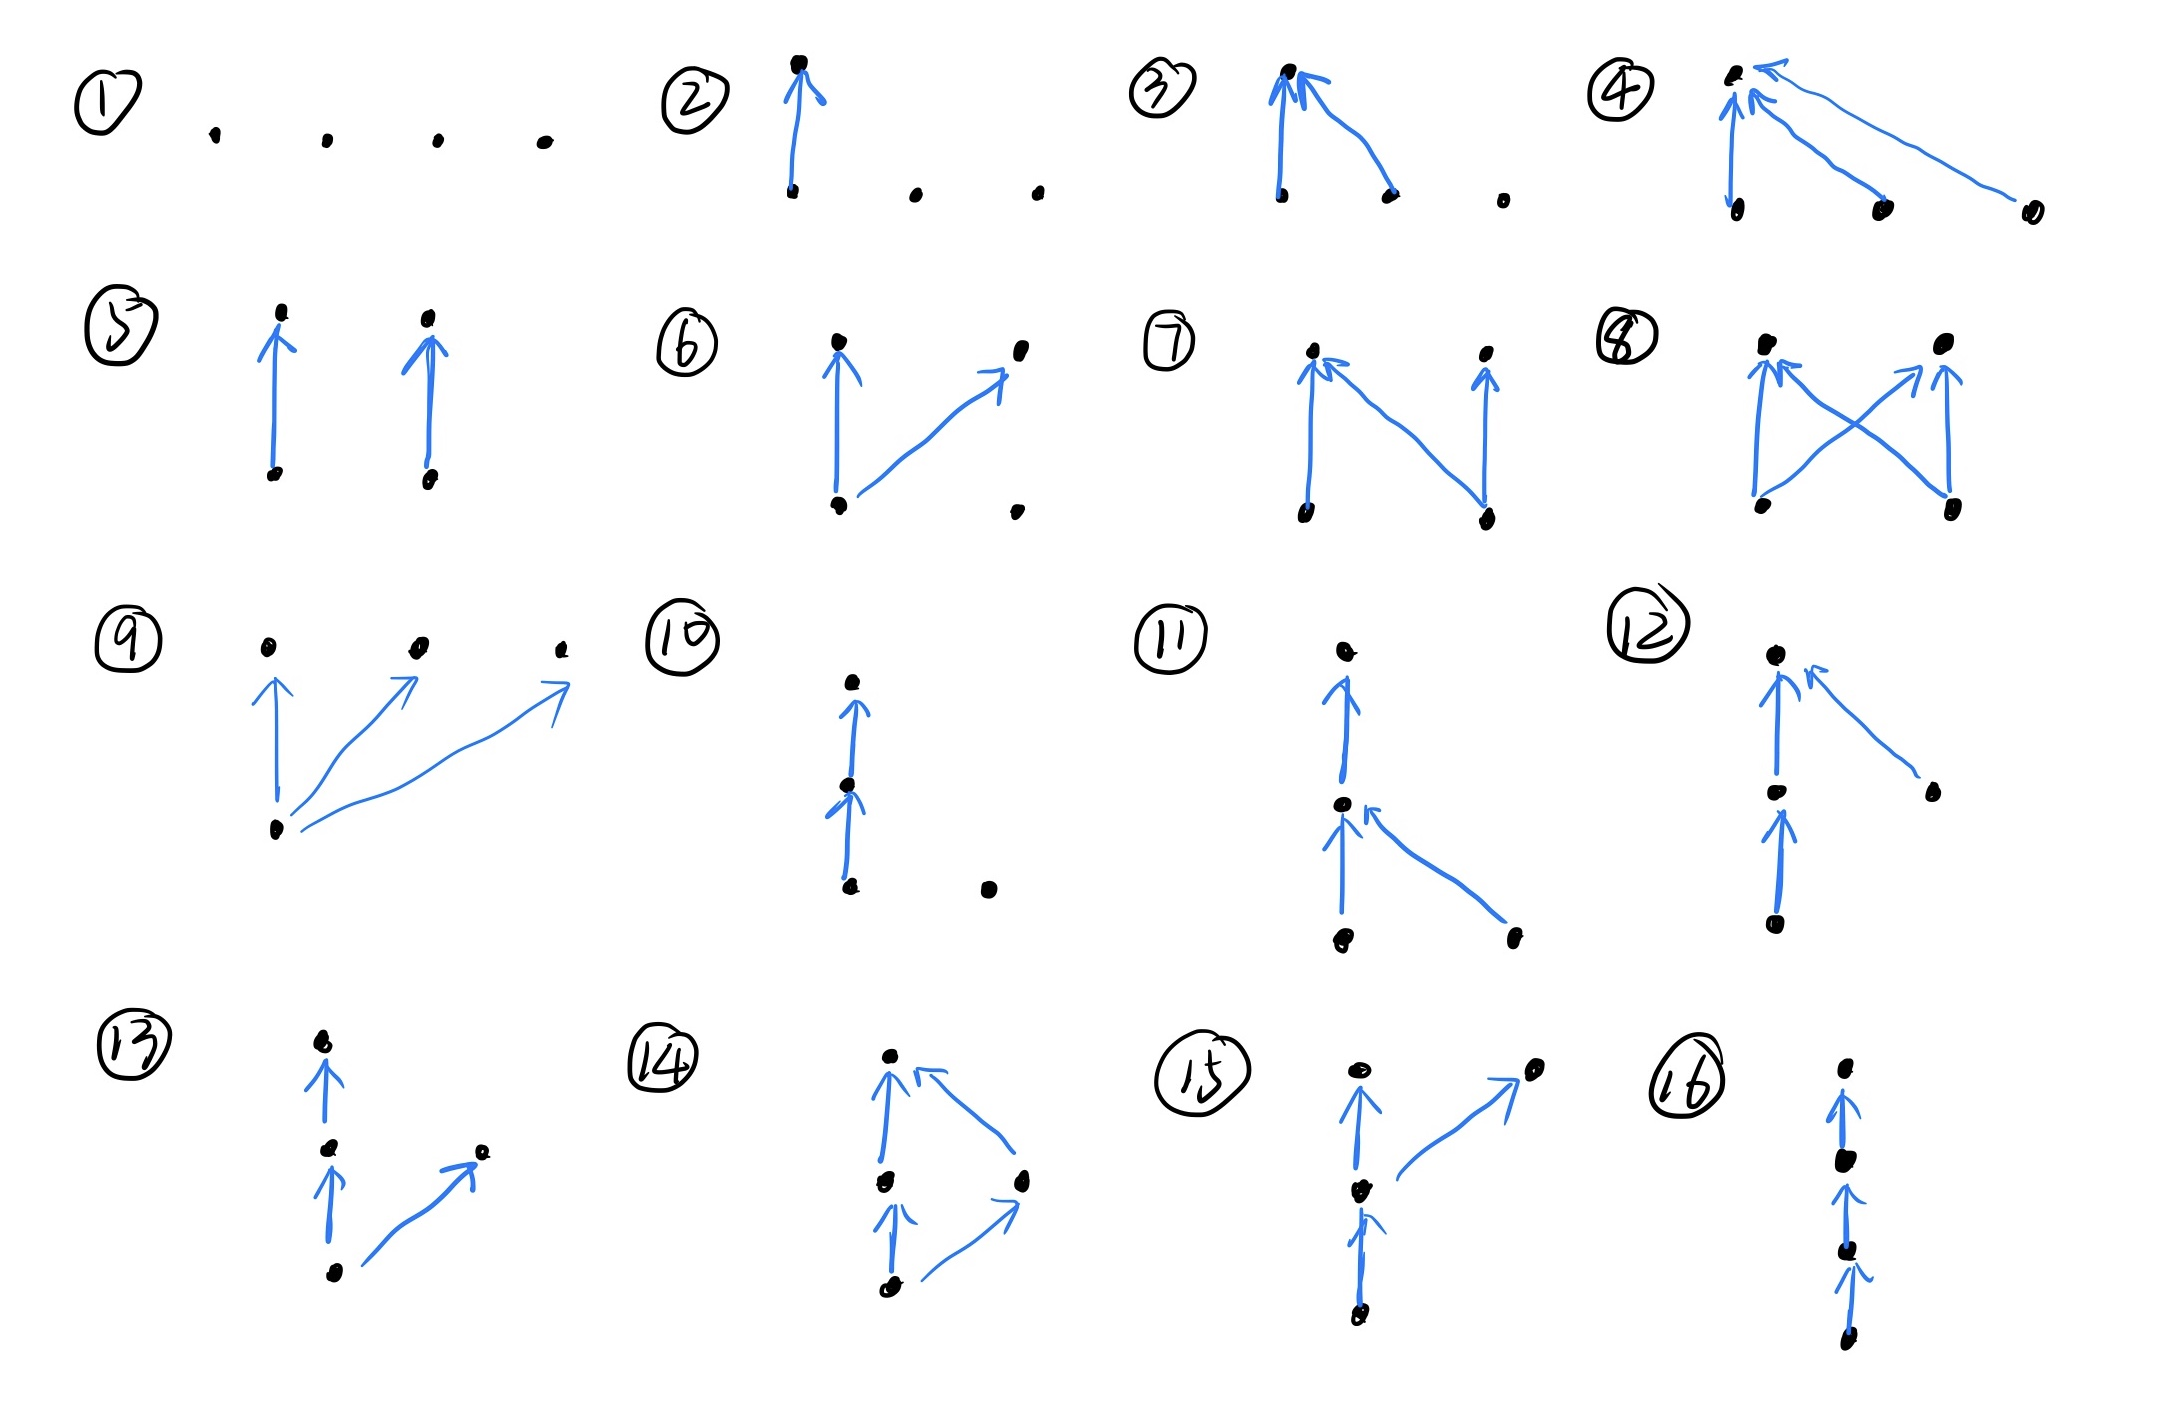
\includegraphics[width=16cm,height=10cm]{Q1.jpg} 
	\end{figure}
	As we can see, 
	\begin{itemize}
	\item 9,13,14,15,16 are chain complete.
	\item 16 is linear order.
	\item 16 is well-order.
	\item 14, 16 are lattices.
	\item 14, 16 are complete lattices.
	\end{itemize}
\noindent \textbf{Q2.}
\begin{enumerate}[(i)]
\item 
If $(L,\preceq)$ is a complete lattice, then $(L,\preceq)$ has a greatest element given by the least upper bound of $L$. Since the greatest element will always be the maximal element and we know that greatest element is unique. Therefore, every complete lattice has a unique maximal element.
\item 
%Let $P=\mathbb{N}\cup(\textbf{a},\textbf{b})$ and define 
%\begin{align*}
%\preceq =&\{(n,n),(n,n+1),(n,\textbf{a}),(n,\textbf{b})\ | \ n\in \mathbb{N}\cup
%\{(\textbf{a},\textbf{a}),(\textbf{b},\textbf{b}))\}
%\end{align*}
The example is ([-10,10] on $\mathbb{R}$,$ \not=^* $), where $\not=^*$ means $\leq$ when $x\geq 0$ and $\not=^*$ means $\geq$ when $x\leq 0$.

Since it is an interval in $\mathbb{R}$, the number of the elements in the interval are infinite. And for $\emptyset$, it has a l.u.b that is 0 since $0\leq$ all the non-negative numbers in the interval and $\geq$ all the non-positive numbers in the interval. And for any non-empty subset (i.e. $(c,d)$, $[c,d)$, $(c,d]$ and $[c,d]$), if it is a chain, $cd\geq 0$. When $c,d$ are all non-negative numbers, the l.u.b of those subset is $d$ and otherwise, it is $c$. Therefore, ([-10,10] on $\mathbb{R}$,$ \not=^* $) is an infinite chain complete poset.\\
However, 10 is greater or equal to any non-negative element in [-10,10] and -10 is less or equal to any non-positive numbers in [-10,10] , so it has no unique maximal element.
\item For any closed interval $[a,b]$ on $\mathbb{R}$, I will show that for every non-empty interval (i.e. $(c,d)$, $[c,d)$, $(c,d]$ and $[c,d]$) $\subseteq [a,b]$, $c$ is the g.l.b and $d$ is the l.u.b of this interval. For the empty set, its l.u.b is $a$ and g.l.b is $b$.
\begin{itemize}
\item For $\emptyset$, every $x\in [a,b]$ can be its upper bound and lower bound. According to the relation ($\leq$), for all $x\in (a.b)$, $x\leq b$ and $a\leq x$. Therefore, $a$ is the l.u.b and $b$ is the g.l.b.
\item For non-empty set,for every $x$ except $c,d$ in the interval between $c$ and $d$, $x< d$ and $c> x$ and $c$ is the g.l.b and $d$ is the l.u.b of this interval. To prove this, we can prove that there is no element $y$ that $y> c$ and for $\forall x\rm{\ in\ the\ interval},\ y\leq x$, by contradiction. And the l.u.b can be proved similarly. [note: if the interval has a closed side, since the relation contains $``="$, it will related to itself. Therefore, the proof above is talking about all the elements except the side.]
\par Suppose there is $y$ that $y> c$ and for $\forall x\rm{\ in\ the\ interval},\ y\leq x$. Because $c< y \leq x$, $c< y < d$ and $y$ must lies in the interval between $c$ and $d$, since all the intervals contains elements that is greater than $c$ and less to $d$. Therefore, from the Calculus class, that we know if $y$ is in the interval, there must exist elements that are still less than $y$, which is contradicted to our assumption.
\end{itemize}
Therefore, any closed interval on $\mathbb{R}\ ([a, b])$ with the usual order ($\leq$) is a complete lattice.
\item The example is ((0,10] on $\mathbb{R}$,$ \leq $). According to the (iii) above, this example is a complete lattice, therefore, it must be almost chain complete. However, there is no element that is less or equal to any element in the interval so there is no minimal element.
\end{enumerate}
\noindent \textbf{Q3.}
The example is listed below, and I omit relationships that are forced by the axioms of reflexivity and transitivity. As we can see, every pair has an upper bound but the bottom pairs don't have a l.u.b.
%The example is ([0,10) on $\mathbb{R}$,$ > $). Every time we have two elements for the interval, any number which is greater than the bigger one of the two elements is an upper bound of the pair. However, since the interval is on the real number, we cannot find the minimal element which is greater than the bigger element in the pair.
\begin{figure}[H]
	\centering
	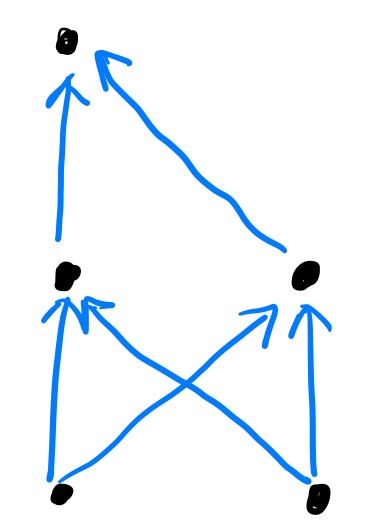
\includegraphics[width=2cm,height=3cm]{Q3.jpg} 
	\end{figure}

\noindent \textbf{Q4.}
\begin{enumerate}
\item Prove that $(\mathbb{N} \times \mathbb{N}, \preceq)$ is a linear order.
\begin{itemize}
\item We first prove that $(\mathbb{N} \times \mathbb{N}, \preceq)$ is a poset
\begin{itemize}
\item We know that $x=x$ and $y\leq y$, thus $(x, y) \preceq(x, y)$. So it is reflexive.
\item Next, for all $x,y,z,w\in \mathbb{N}$, if $(x, y) \preceq(z, w)$ and $(z, w) \preceq(x, y)$, we know that first $x<z$ or $(x=z$ and $y \leq w)$ and second $z<x$ or $(z=x$ and $w \leq y)$. For the relation between $x$ and $z$, only when $x=z$ can satisfy both requirements. For the relation between $y$ and $w$, to satisfy both requirements, we need to have $y\leq w$ and $w\leq y$, which implies that $y=w$. Therefore, we prove that it is antisymmetric.
\item Then, suppose $(x, y) \preceq(z, w)$ and $(z, w) \preceq(a, b)$, then we have first $x<z$ or $(x=z$ and $y \leq w)$ and second $z<a$ or $(z=a$ and $w \leq b)$. If $x<z$ or $x=z$ but $z<a$, then we always have $x<a$, and then $(x, y) \preceq(a, b)$. If $x=z=a$, since we always have $y\leq w\leq b$, and then $(x, y) \preceq(a, b)$. Therefore, it is transitive.
\end{itemize}  
\item We prove that it is a linear order by showing if for all $x,y,z,w\in \mathbb{N}$, $(x, y) \not\preceq(z, w)$, we must have $(z, w) \preceq(x, y)$. Since if $(x, y) \not\preceq(z, w)$, either $x>z$ or ($x=z$ and $y>w$). These two conditions ensure that $z<x $ or $(z=x$ and $w \leq y)$, which means $(z, w) \preceq(x, y)$.
\end{itemize}
\item Yes, it is a well-order. Since $(\mathbb{N}, \leq)$ is a well-order, for any non-empty $A\subseteq \mathbb{N}$, we have an element that is less to any other element in the $\mathbb{N}$ and equal to itself. Therefore, we have either $x<z$ and $x\not=z$ for any other $z\in \mathbb{N}$, or $x=x$.
Due to the same reason, we can also find a $y$ such that $y\leq w$ for every $w\in \mathbb{N}$.
Therefore, for this subset $A$, we can always find a $(x,y)\in A$, such that for all $(z,w)\in A$, such that either $x$ is always less than $z$, or $x=z$ but we have $y\leq w$.
\end{enumerate}


\noindent \textbf{Q5.}
\begin{enumerate}
\item Prove that $(\mathbb{N} \times \mathbb{N}, \preceq)$ is a poset.
\begin{itemize}
\item We know that $x\leq x$ and $y\leq y$, thus $(x, y) \preceq (x, x)$. So it is reflexive.
\item Next, for all $x,y,z,w\in \mathbb{N}$, if $(x, y) \preceq(z, w)$ and $(z, w) \preceq(x, y)$, we know that first $x\leq z$ and $y \leq w$, and second $z\leq x$ and $w \leq y$. For the relation between $x$ and $z$, to satisfy both requirements, we need to have $x\leq z$ and $z\leq x$, which implies $x=z$. Similarly, $y=w$. Therefore, we prove that it is antisymmetric.
\item Then, suppose $(x, y) \preceq(z, w)$ and $(z, w) \preceq(a, b)$, then we have first $x\leq z$ and $y \leq w$, and second $z\leq a$ and $w \leq b$. Therefore, we have $x\leq z\leq a$ and $y\leq w\leq b$, and thus $(x, y) \preceq(a, b)$. Therefore, it is transitive.
\end{itemize}  
\item No, it isn't a linear order. For $x,y,z,w\in \mathbb{N}$, if $(x, y) \not\preceq(z, w)$, either $x>z$ or $y>w$. These two conditions cannot ensure that $z\leq x$ and $y\leq w$ for the same time. Therefore, we cannot conclude that $(z, w) \not\preceq(x, y)$. Therefore, it isn't a linear order.
\item Yes, it is a lattice. For all $(x,y),(z,w)\in \mathbb{N}\times \mathbb{N}$, the set \{$(x,y),(z,w)$\} has both a l.u.b and a g.l.b, where $(x,y)\vee(z,w)=(\max(x,z),\max(y,w))$ and $(x,y)\wedge(z,w)=(\min(x,z),\min(y,w)$
\end{enumerate}

\noindent \textbf{Q6.}
$(\mathbb{Q}\times \mathbb{Q} \times \mathbb{Q},  \preceq)$ is not a poset. We can prove it by showing that it is not antisymmetric.
%\begin{itemize}
%\item We know that $x\leq x$, thus $(x, y,p) \preceq (x, y,q)$. So it is reflexive.
%\item 
For $x,y,z,w\in \mathbb{Q}$, if $(x, y,p) \preceq(z, w,q)$ and $(z, w,q) \preceq(x, y,p)$, we know that first $x\leq z$ or ($y \leq w$ and $p\leq q$, and second $z\leq x$ or ($w \leq y$ and $q\leq p$). For the relation between $x$ and $z$, it is possible that $x<z$ to make $(x, y,p) \preceq(z, w,q)$. Therefore, to make $(z, w,q) \preceq(x, y,p)$, we must ensure that $w \leq y$ and $q\leq p$. It is possible that $w<y$ and $q<p$. Therefore, we have two different element in $\mathbb{Q}\times \mathbb{Q} \times \mathbb{Q}$ such that they are related to each other by the relation $\preceq$. Therefore, it isn't antisymmetric.
\\



%\item Then, suppose $(x, y) \preceq(z, w)$ and $(z, w) \preceq(a, b)$, then we have first $x\leq z$ and $y \leq w$, and second $z\leq a$ and $w \leq b$. Therefore, we have $x\leq z\leq a$ and $y\leq w\leq b$, and thus $(x, y) \preceq(a, b)$. Therefore, it is transitive.
%\end{itemize}  
\noindent \textbf{Q7.}
\begin{enumerate}
\item Prove that $\sim$ is an equivalence relation on \textit{A}.
\begin{itemize}
\item For all $x\in A$, because $f$ is a function, we have $f(x)-f(x)$. Therefore. Therefore, we have $x\sim x$ and $\sim$ is reflexive.
\item For all $x,y\in A$, if $x\sim y$, then $f(x)=f(y)$. And then $f(y)=f(x)$ leads to $y\sim x$, which verifies the relation is symmetric.
\item For all $x,y,z\in A$, if $x\sim y$ and $y\sim z$, we have $f(x)=f(t)$ and $f(y)=f(z)$, which leads to $f(x)=f(z)$. Therefore, $x\sim z$ and we prove the transitive property.
\end{itemize}
\item Prove that \textit{g} is a function:\\
Suppose for all $[x]_{\sim}\in X$, $a,b\in B$, $([x]_{\sim},a)\in g$ and $([x]_{\sim},b)\in g$. According to $g\left([x]_{\sim}\right)=f(x)$, $a=f(x)$ and $b=f(x)$. Since $f(x)$ is a function, the value of $f(x)$ is unique. Therefore, $a=b$. So $g$ is a function.
\item Prove that \textit{g} is injective:\\
Suppose for all $[x]_{\sim},[y]_{\sim}\in X$, $a\in B$, $g\left([x]_{\sim}\right)=a=f(x)$ and $g\left([y]_{\sim}\right)=a=f(y)$. Therefore, $f(x)=f(y)$, which means $x\sim y$ and therefore $y\in [x]_{\sim}$. Because $y\in [y]_{\sim}$, $[x]_{\sim}\cap [y]_{\sim}\not=\emptyset$. So $[x]_{\sim}=[y]_{\sim}$. Therefore, $g$ is injective.
\item For the function $f:\mathbb{R} \longrightarrow \mathbb{R}$ defined by $f(x) = x^3- 4x^2-15x + 18$, find all the elements of $g^{-1}$(0).\\
We first calculate $f(x)=0$ and find that $x=6,1,-3$. Therefore, he elements of $g^{-1}(0)$ is $[6]_{\sim}, [1]_{\sim}, [-3]_{\sim}$.
\end{enumerate}
\noindent \textbf{Q8.}
\begin{enumerate}[(i)]
\item \begin{align*}
&(\exists x P(x) \wedge \exists y Q(y)) \Rightarrow \exists z(P(z) \wedge Q(z))\\
\equiv &\neg (\exists x P(x) \wedge \exists y Q(y)) \vee \exists z(P(z) \wedge Q(z))\\
\equiv &\neg (\exists x P(x))\vee \neg (\exists y Q(y)) \vee \exists z(P(z) \wedge Q(z))\\
\equiv &(\forall x \neg P(x)) \vee (\forall y \neg Q(y))\vee \exists z(P(z) \wedge Q(z))\\
\equiv & (\neg P(z))\vee (\neg Q(z))\vee (P(z)\wedge Q(z)),\exists z\\
\equiv & ((\neg P(z))\vee (\neg Q(z))\vee P(z))\wedge ( (\neg P(z))\vee (\neg Q(z))\vee Q(z)),\exists z\\
\equiv & (\neg Q(z))\wedge (\neg P(z)),\exists z\\
\not\equiv &T
\end{align*}
%,\rm{when\ \textit{Q(z)}\equiv \textit{ T}\ but\ \textit{P(z)}\equiv \textit{F}\ for\ example}
\item 
\begin{align*}
&(\forall z(Q(z) \vee P(z))) \Rightarrow((\forall x Q(x)) \vee(\forall y P(y)))\\
\equiv & \neg (\forall z(Q(z) \vee P(z)))\vee ((\forall x Q(x)) \vee(\forall y P(y)))\\
\equiv &(\exists z \neg (Q(z) \vee P(z)))\vee ((\forall x Q(x)) \vee(\forall y P(y)))\\
\equiv & (\exists z (\neg Q(z)\wedge \neg P(z)))\vee ((\forall x Q(x)) \vee(\forall y P(y)))\\
\equiv & (\neg Q(z)\wedge \neg P(z))\vee ( Q(z) \vee P(z)),\exists z\\
\equiv &(\neg Q(z)\vee  Q(z) \vee P(z)) \wedge (\neg P(z)\vee  Q(z) \vee P(z)),\exists z\\
\equiv &P(z)\wedge Q(z) ,\exists z\\
\not\equiv &T
\end{align*}
%,\rm{when\ \textit{Q(z)}\equiv \textit{T}\ but\ \textit{P(z)}\equiv \textit{F}\ for\ example}
\item 
\begin{align*}
&((\forall x P(x)) \Rightarrow(\exists y Q(y))) \Rightarrow \forall z(P(z) \Rightarrow \exists w Q(w))\\
\equiv & \neg ((\forall x P(x)) \Rightarrow(\exists y Q(y))) \vee \forall z(P(z) \Rightarrow \exists w Q(w))\\
\equiv & \neg (\neg (\forall x P(x)) \vee (\exists y Q(y))) \vee \forall z(\neg P(z) \vee \exists w Q(w))\\
\equiv & ((\forall x P(x))\wedge (\exists y Q(y)) )\vee \forall z(\neg P(z) \vee \exists w Q(w))\\
\equiv & ((\forall x P(x))\vee  (\forall z\neg P(z)) \vee (\exists w Q(w)))\wedge ((\exists y Q(y))\vee (\forall z\neg P(z) )\vee (\exists w Q(w)))\\
\equiv & (\exists w Q(w)) \wedge ((\forall z\neg P(z) )\vee (\exists w Q(w)))\\
\equiv & \exists w Q(w)\\
\not\equiv & T
\end{align*}
\end{enumerate}
%, 
%\rm{when\ \textit{Q(w)}\equiv \textit{F}\ for\ example}

\noindent \textbf{Q9.}
\begin{enumerate}
\item $\exists x(\neg Q(x))$ is a premise.
\item $\neg Q(a)$, where $a$ is some (unknown) element of the domain of discourse, by Existential Instantiation.
\item $\forall x(P(x) \vee Q(x))$ is a premise.
\item $P(a) \vee Q(a)$ by Universal Instantiation of (3).
\item $P(a)$ by Identity for $\vee$ of (2) and (4).
\item $\forall x(R(x) \Rightarrow \neg P(x))$ is a premise.
\item $R(a) \Rightarrow \neg P(a)$ by Universal Instantiation of (6).
\item $P(a)\Rightarrow \neg R(a)$ by contraposition of (7).
\item $\neg R(a)$ by Modus Ponens from (5) and (8).
\item $\exists x(\neg R(x))$ by Existential Generalisation of (9).
\end{enumerate}


\noindent \textbf{Q10.}
The green one will lead A. and B. to safety. 
Since the blue one and the green one say the same thing, they should share the same truth or falsehood. And given that at least one is true and at least one is false, the truth or falsehood of statement on the red door is opposite from those two doors.\\
\begin{enumerate}
\item Suppose the statement on Red door is true and on the other two are false. The freedom is behind both the red door and the blue door, which is wrong.
\item Suppose the statement on Red door is false and on the other two are true. The freedom is behind neither the red door nor the blue door. Therefore, it should be behind the green door.
\end{enumerate}










%========================================================================
\end{document}
